\documentclass[../informe_krapp.tex]{subfiles}
\begin{document}
\section{Gabinete diseñado en 3D}
El diseño 3D fue hecho en Tinkercad, el cual se puede encontrar aquí \small{\url{ https://www.tinkercad.com/things/agi002oQ6x5 }}

\begin{figure}[H]
	\centering
	% Imagenes de la primera fila
	\begin{subfigure}[b]{0.49\textwidth}
		\centering
		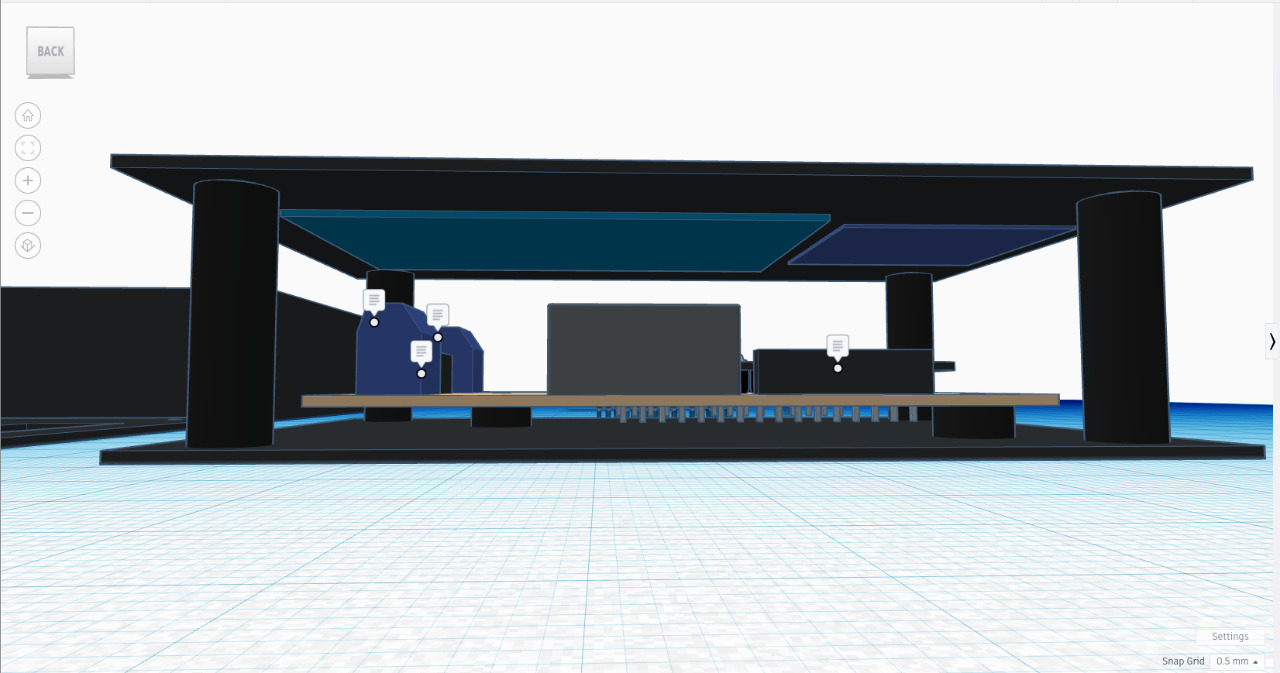
\includegraphics[width=\textwidth]{gabinete-1}
	\end{subfigure}
	\hfill
	\begin{subfigure}[b]{0.49\textwidth}
		\centering
		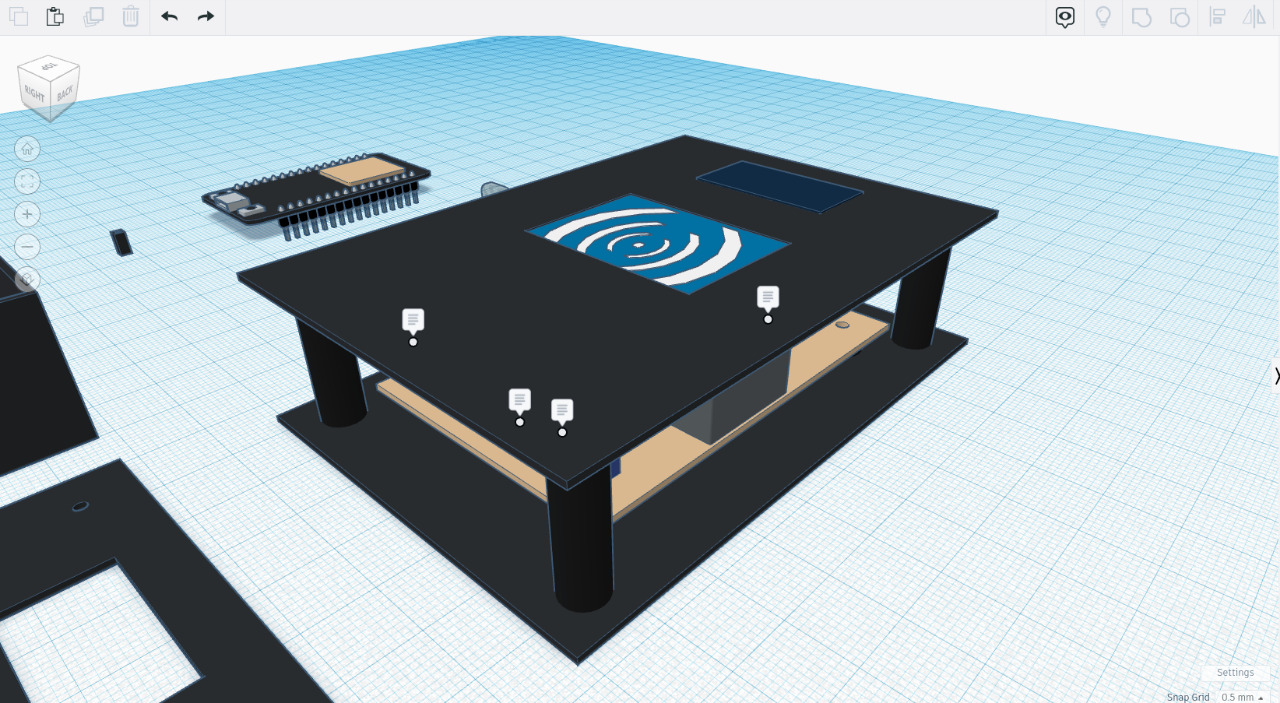
\includegraphics[width=\textwidth]{gabinete-2}
	\end{subfigure}

	% Imagenes de la segunda fila
	\begin{subfigure}[b]{0.49\textwidth}
		\centering
		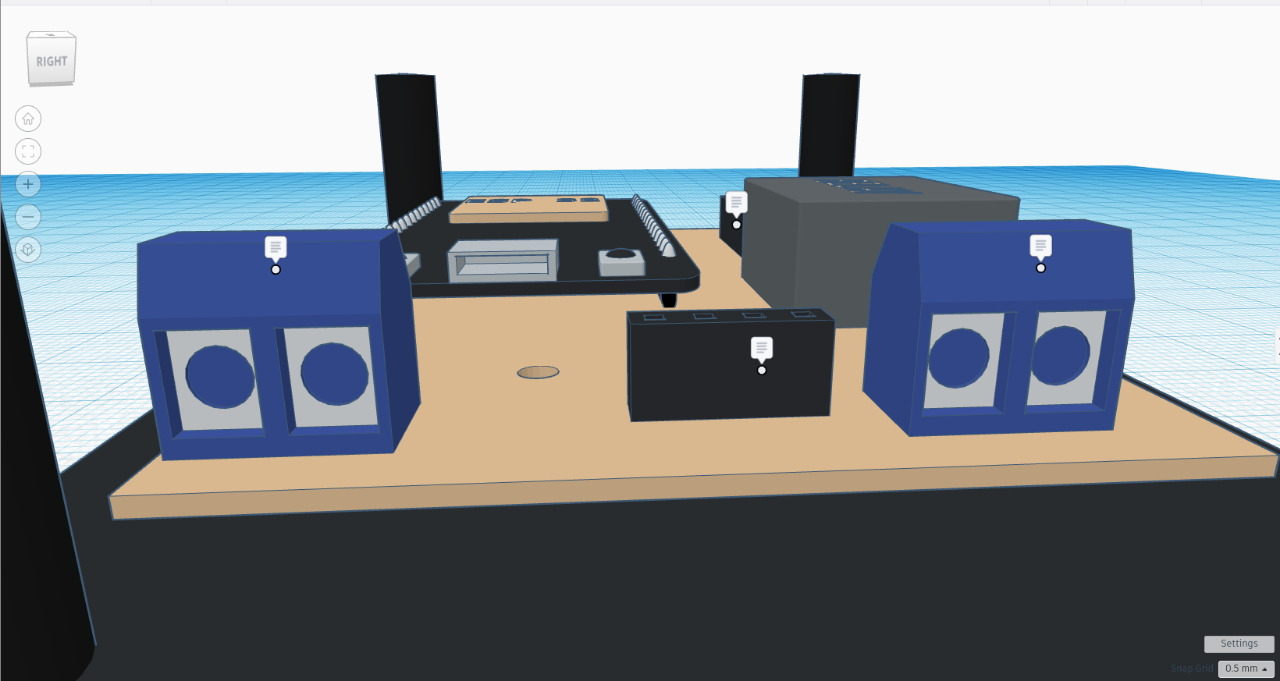
\includegraphics[width=\textwidth]{gabinete-3}
	\end{subfigure}
	\hfill
	\begin{subfigure}[b]{0.49\textwidth}
		\centering
		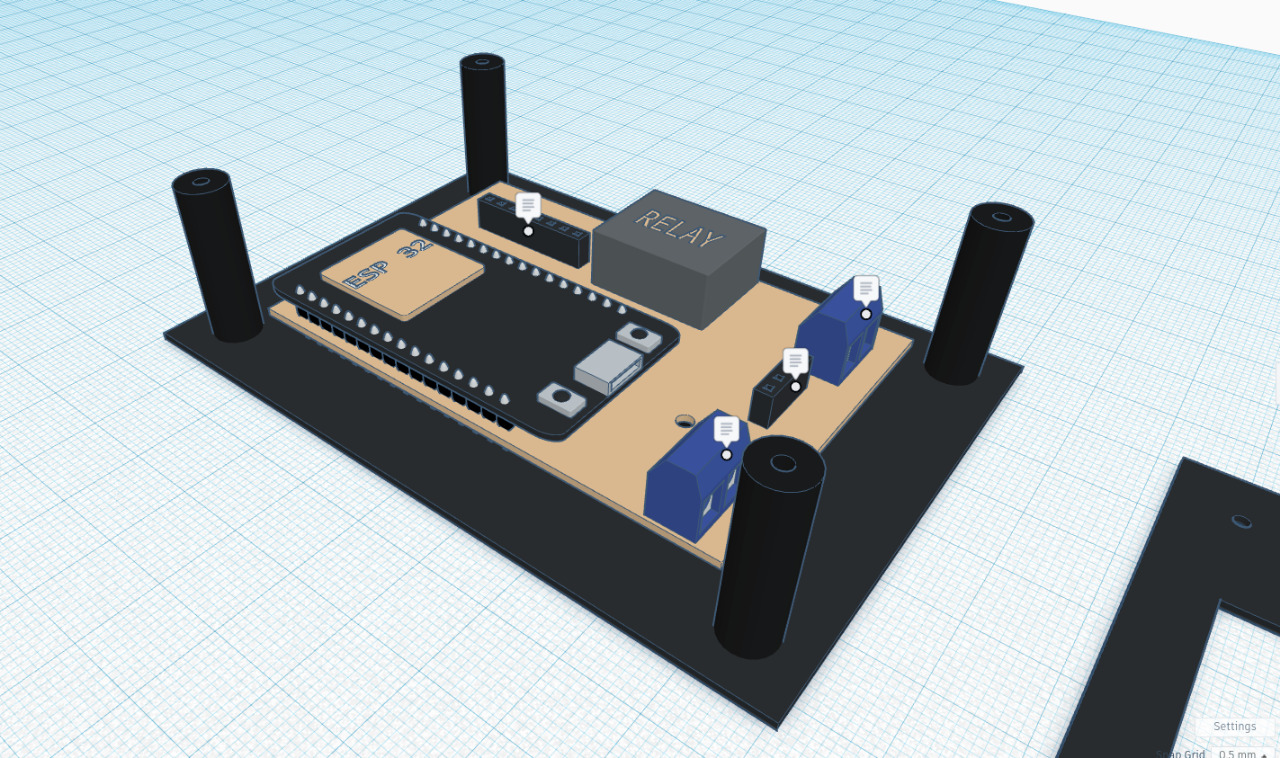
\includegraphics[width=\textwidth]{gabinete-4}
	\end{subfigure}

	% Imagenes de la tercera fila
	\begin{subfigure}[b]{0.49\textwidth}
		\centering
		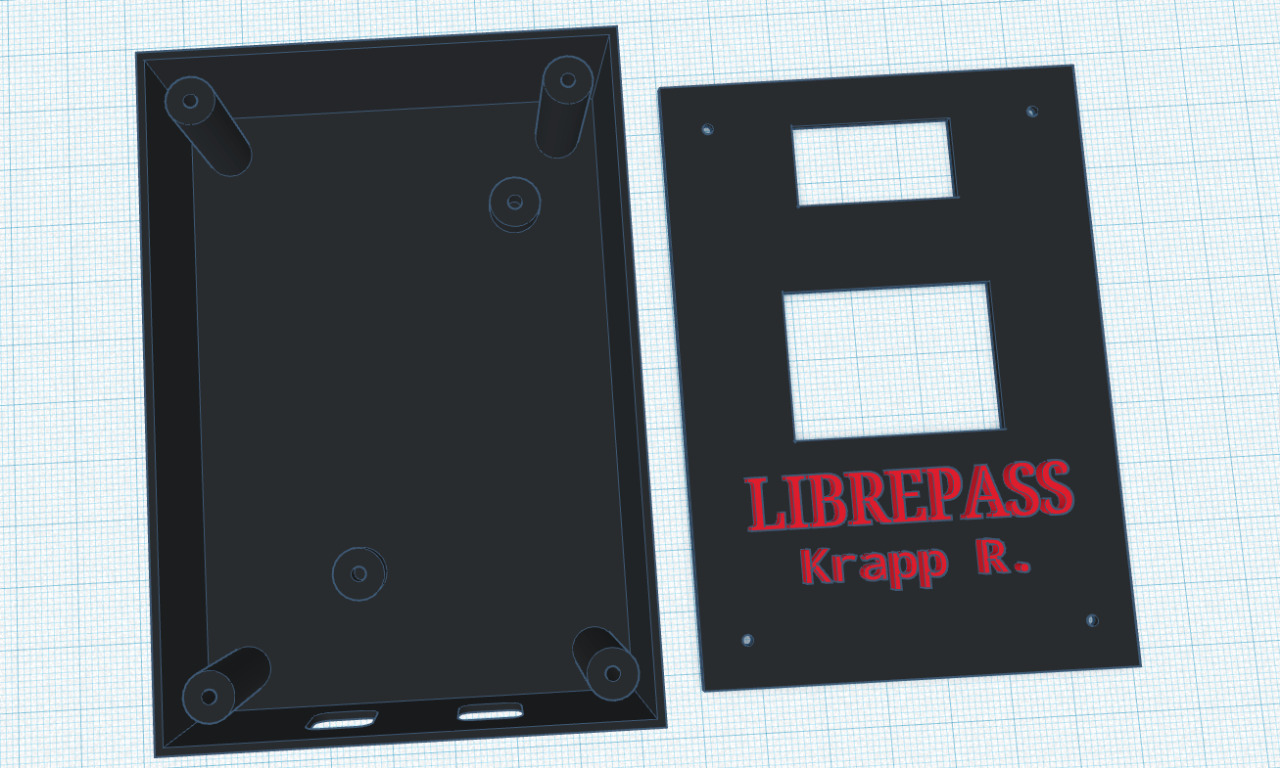
\includegraphics[width=\textwidth]{gabinete-5}
	\end{subfigure}
	\hfill
	\begin{subfigure}[b]{0.49\textwidth}
		\centering
		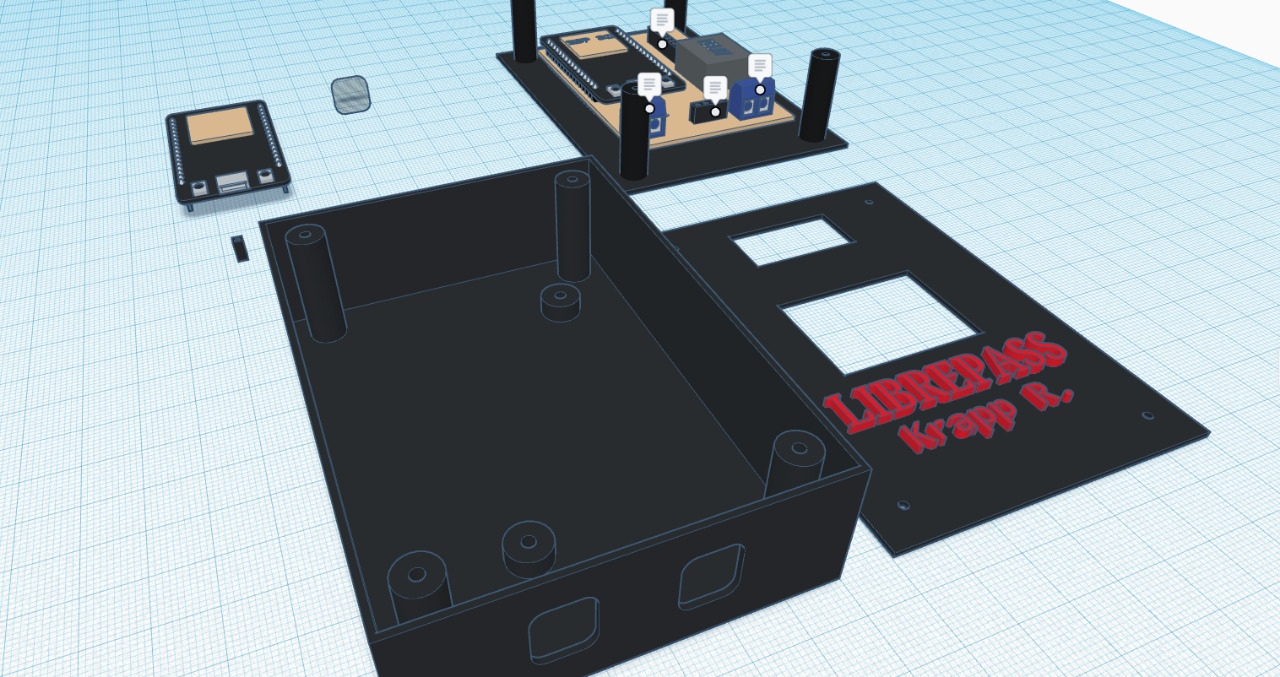
\includegraphics[width=\textwidth]{gabinete-6}
	\end{subfigure}
	\caption{Capturas de pantalla del diseño en 3D}
\end{figure}
\end{document}